\section{Metodologia}
\begin{onehalfspace}
    Assim, neste capítulo são apresentadas as três principais etapas utilizadas na 
metodologia para esta pesquisa. Estas etapas podem ser descritas como:
\begin{easylist}
    \ListProperties(Numbers1=r,Numbers2=l,Hide2=1,Hang=true,Margin1=3ex,Margin2=6ex,FinalSpace=1em)
    @ Definição dos modelos genéricos. A etapa de definição dos modelos foi elaborada em 3 partes, 
    dentre as quais:
        @@ Coleta    de    dados    sobre    as    características    das    edificações    comerciais, 
        especificamente de escritório, em Vitória (ES);
        @@ Levantamento e definição das variáveis sobre os padrões de uso e ocupação das 
        salas  de  escritório,  assim  como  padrões  de  conforto  e  níveis  de  
        eficiência energética dos equipamentos de condicionamento de ar e iluminação;
        @@ Estabelecimento  dos  modelos  genéricos com  o  intuito de  evidenciar o  
        consumo total  final  de  energia  elétrica  por  meio  da  determinação  da  classe  
        de  eficiência energética  da  edificação,  proposta  pela  INI-C,  e  o  
        potencial  de  otimização  e produção de energia elétrica a partir de fontes renováveis.
    @ Simulações.  Nesta  etapa  são  avaliadas  as  características  mais  influentes  
    no  consumo energético da edificação de referência e o potencial de geração de energia 
    solar. Ambas as  avaliações  serão  feitas  por  meio  de  simulação  computacional.  
    As  simulações  foram fracionadas em 3 partes, dentre as quais:
        @@ Simulação dos modelos real e de referência, onde é feita a determinação da classe 
        de desempenho energético das edificações observadas em campo; 
        @@ Otimização    dos    modelos    genéricos,    representando    a    etapa    onde    
        são implementadas estratégias passivas e ativas visando a eficientização da edificação;
\end{easylist}
\vspace*{0.3cm}
\noindent Com a aplicação da metodologia, simplificada no Fluxograma da Figura \ref{fig:figura7}, busca-se identificar se há 
condições para o balanço energético nulo total ou parcial dos modelos analisados.
\begin{figure}[ht]
    \centering
    \footnotesize
    \caption{\small Esquema simplificado da metodologia criada.}
    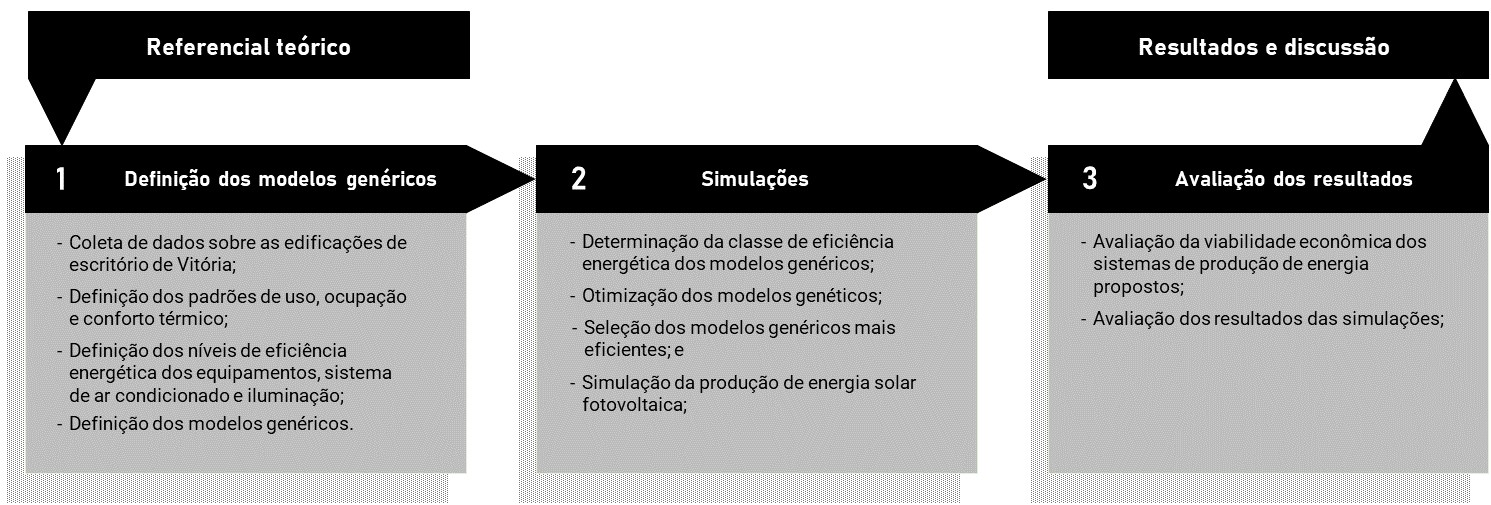
\includegraphics[width=1\textwidth]{figures/fig8_Fluxogramas_1.jpg}
    \begin{flushleft}
        \par \small Fonte: autor (2019).
    \end{flushleft}
    \label{fig:figura7}
\end{figure}\vspace*{-0.3cm}
\subsection{Levantamento das características dos edifícios de escritório de Vitória}
As edificações de escritório de Vitória selecionadas após a definição do recorte 
territorial, apresentam características que foram complementadas aos atributos 
observados em edificações comerciais brasileiras, como suporte as informações não 
encontradas in loco. As características com maior frequência de ocorrência no 
levantamento realizado são apresentadas na Tabela \ref{tab:tabela4}. Todavia, a amostra coletada 
abrange edifícios iniciados em 2003 e concluídos até o fim do primeiro trimestre 
de 2018, data do início do levantamento. Este fato inviabiliza aplicar a última 
revisão do Plano à amostra.\vspace*{0.3cm} \newline
Foram considerados para o levantamento atributos como gabarito, número de 
pavimentos-tipo, número de salas por pavimento-tipo, dimensão e forma, altura 
dos pavimentos-tipo. Não foram consideradas as dimensões dos lotes onde as 
edificações da amostra estacam implantadas, já que este atributo não foi 
pertinente ao objetivo do trabalho. Estes parâmetros foram reunidos em consulta 
ao material técnico disponibilizado pelas construtoras, visitas a campo e 
complementação de dados utilizando a ferramenta computacional \textit{Google Street View}.\vspace*{0.3cm} \newline
Os trabalhos de \textcite{Lamberts2006,AmericanSocietyofHeatingRefrigeratingandAir-ConditioningEngineers-ASHRAE2010,Bernabe2012,Ramos2013,Didone2014,Didone2014a,ConselhoBrasileirodeConstrucaoSustentavel-CBCS2015,Fonseca2016,Werneck2017,InstitutoNacionaldeMetrologiaNormalizacaoeQualidadeIndustrial-INMETRO2018},
foram utilizados como principais fontes de informação para a análise de envoltória 
e sistema de iluminação e condicionamento de ar.\vspace*{-0.6cm}
\begin{table}[ht]\centering
    \caption{\small Características observadas em campo e em pesquisas anteriores.}
    \vspace*{0.2cm}
    \label{tab:tabela4}
    \begin{tabular*}{\columnwidth}{@{\extracolsep{\fill}}lll}
    \hline
    \textbf{Parâmetro}                                             & \textbf{Descrição}                                                                    & \textbf{Referências} \\ \hline
    Gabarito                                                       & 24 a 60 m (8 a 19 pav.)                                                               & \makecell[l]{Levantamento \textit{in loco} e referências\\ (BERNABÉ, 2012; CBCS, 2015; \\FONSECA et al., 2016; LAMBERTS; \\GHISI; RAMOS, 2006; RAMOS \\et al., 2013).} \\ \hline
    Altura do pavimento                                            & 3 m                                                                                   & Levantamento \textit{in loco}.                                                                                                                                         \\ \hline
    Planta-baixa (forma)                                           & Retangular                                                                            & \makecell[l]{Levantamento \textit{in loco} e referências\\ (FONSECA et al., 2016; INMETRO,\\ 2018).}                                                                   \\ \hline
    \makecell[l]{Dimensão das salas\\ por pav.-tipo}               & 40 m²                                                                                 & \makecell[l]{Foi fixado a área das salas \\(zonas térmicas) de acordo com a \\média de ofertas de salas observadas\\ em levantamento \textit{in loco}.}                  \\ \hline
    \multicolumn{3}{c}{Continua}\\\hline
    \end{tabular*}
\end{table}\pagebreak
\begin{table}[ht]\centering
    \begin{tabular*}{\columnwidth}{@{\extracolsep{\fill}}lll}
    \hline
    \multicolumn{3}{c}{Conclusão}\\\hline
    \makecell[l]{Componentes da\\ parede}                          & \makecell[l]{Bloco cerâmico,\\ 8 furos; \\14x19x29 cm; \\argamassa de\\ assentamento} & Levantamento \textit{in loco}.                                                                                                                                         \\ \hline
    Proteção solar                                                 & Sem proteção                                                                          & \makecell[l]{Levantamento \textit{in loco} e referências\\ (FONSECA et al., 2016; WERNECK \\et al., 2017).}                                                            \\ \hline
    Cobertura                                                      & \makecell[l]{Laje impermeabilizada\\ com 20 cm de\\ espessura}                        & \makecell[l]{Levantamento \textit{in loco} e referências \\(CB3E; ABIVIDRO, 2015).}                                                                                    \\ \hline
    Vidros                                                         & \makecell[l]{Laminado; Reflexivo;\\ 8 mm; Verde}                                      & \makecell[l]{(FONSECA et al., 2016; \\INMETRO, 2018).}                                                                                                                   \\ \hline
    PAF\textsubscript{T}                                           & 30\%; 50\%; 80\%                                                                      & \makecell[l]{Levantamento \textit{in loco}\\ e referências.}                                                                                                             \\ \hline
    \makecell[l]{Orientação solar da \\fachada principal}          & Sul                                                                                   & \makecell[l]{Levantamento \textit{in loco}\\ e referências.}                                                                                                             \\ \hline
    \makecell[l]{Densidade de Carga de\\ Iluminação Limite – DCIL} & 14,1 W/m²                                                                             & \makecell[l]{Consulta pública do RTQ-C \\(INMETRO, 2018).}                                                                                                               \\ \hline
    \makecell[l]{Densidade de Carga de\\ Equipamentos – DCE}       & 9,7 W/m²                                                                              & \makecell[l]{Consulta pública do RTQ-C \\(INMETRO, 2018).}                                                                                                               \\ \hline
    \makecell[l]{Absortância/transmitância \\das paredes}          & \makecell[l]{0,59 (cor \\camurça)/3,75}                                               & \makecell[l]{Valores consultados na \\NBR 15220-2 e referências \\(ABNT, 2003; FONSECA et \\al., 2016; INMETRO, 2018).}                                                                     \\ \hline
    \makecell[l]{Absortância/transmitância \\das coberturas}       & \makecell[l]{0,65 (concreto \\aparente)/2,06}                                         & \makecell[l]{Valores consultados na \\NBR 15220-2 e referências \\(ABNT, 2003; FONSECA et \\al., 2016; INMETRO, 2018).}                                                 \\ \hline
    \end{tabular*}
    \begin{flushleft}
        \par \small Fonte: autor (2019).
    \end{flushleft}
\end{table}\vspace*{-0.3cm}

\noindent As informações coletadas nos estudos e em levantamento formam a base conceitual para 
determinar os aspectos arquitetônicos relevantes para compor os modelos genéricos e, 
posteriormente, determinar os parâmetros de otimização e do consumo energético padrão 
aproximado para um edifício de escritório. Além disso, a quantidade de simulações necessárias 
para determinar o consumo de energia dos modelos genéricos é identificada por meio da 
organização dos dados coletados em campo e, assim, a resultante do número de variáveis.

\subsubsection{Consumo de energia elétrica das edificações}
\noindent O consumo de energia elétrica em edificações de escritório no Brasil é determinado 
principalmente por sua tipologia. As configurações predominantes no Brasil compreendem, em 
sua maioria, pequenas edificações, abaixo de 8 pavimentos, a edifícios grandes, acima de 
15 pavimentos \cite{Carlo2008,Ramos2013,ConselhoBrasileirodeConstrucaoSustentavel-CBCS2015,Fonseca2016}.\vspace*{0.3cm} \newline
\noindent Correlacionado às tipologias arquitetônicas, os dados de consumo de energia, expressos em 
Intensidade de Uso de Energia – IUE, kWh/m²/ano, foram necessários para validação das 
simulações iniciais quanto ao consumo de energia esperado dos modelos. Visto que a calibração 
dos modelos genéricos não foi possível, pois eles não dispunham de memorial de massa como 
ferramenta de comparação ao consumo simulado computacionalmente, foram adotados como método 
de comparação os valores médios registrados no Relatório Final do CBCS (2015), como mostra o 
Histograma no Gráfico 5. Foi relacionado o consumo de energia das edificações levantadas à 
frequência de ocorrência da quantidade de pavimentos de edificações comerciais brasileiras e 
suas respectivas áreas comuns.

    \begin{graph}
        \par \small Gráfico 5 - Consumo energético em edificações de escritório brasileiras.
        \begin{minipage}[ht]{1\textwidth}\centering
            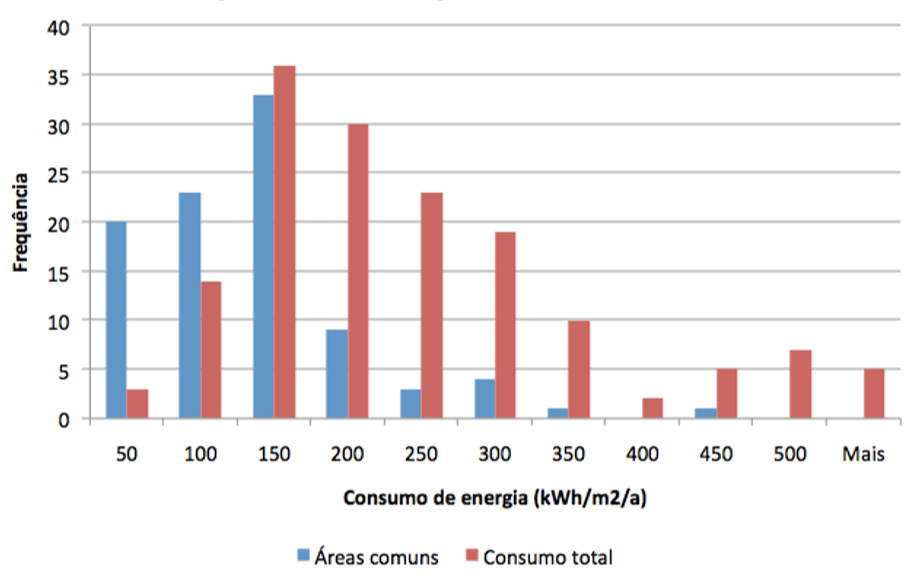
\includegraphics[width=0.85\textwidth]{figures/fig9_consumo-total-das-edificacoes-levantadas_cbcs_2015.png}            
        \end{minipage}
        \begin{flushleft}
            \par \small Fonte: adaptado de CBCS (2015).
        \end{flushleft}
    \end{graph}

\noindent Logo, os dados de IUE adotados para a comparação e avaliação inicial do consumo energético dos 
modelos foram baseados nos valores máximo e mínimo estabelecidos pelo CBCS (2015). A média 
entre o consumo em áreas comuns e total relacionado à frequência de quantidade de pavimentos 
define a quantidade total de consumo de energia para cada tipologia.\vspace*{0.3cm} \newline
Os autores do Relatório atribuem 133 kWh/m²/ano aos edifícios de pequeno porte, e 
268 kWh/m²/ano às edificações de grande porte. Vale ressaltar que os dados de consumo 
energético, assim como a média apontada no Relatório, de 191 kWh/m²/ano, desprezam as 
distorções causadas por edificações com particularidades de consumo como datacenters ou erros 
de cálculo de área útil.\vspace*{0.3cm} \newline
Ao estabelecer as Intensidades de Uso de Energia equivalentes a cada modelo, assim como os 
padrões de uso e ocupação, pode-se estimar o consumo de energia durante determinado período.

\subsubsection{Padrões de uso e ocupação em edifícios de escritório}
Os padrões de uso e ocupação da edificação foram baseados em normas, regulamentos, relatórios 
técnicos e referências acadêmicas que consideraram os níveis de atividades desenvolvidas nos 
ambientes, tratadas neste trabalho como zonas térmicas, como apresentado na Tabela \ref{tab:tabela5}.\vspace*{0.3cm} \newline
Como o intuito do trabalho foi criar modelos genéricos que representassem minimamente o 
cenário encontrado na cidade de Vitória, as características de uso e ocupação escolhidas 
foram integradas como forma de aproximar as tipologias ao cenário observado. Dentre elas, 
pode-se citar:
\begin{itemize}
    \item O nível metabólico apresentado em atividades de escritório;
    \item O horário de funcionamento dos escritórios, determinando os intervalos de tempo de ocupação total e parcial, onde, respectivamente, a capacidade máxima e parcial de ocupação das zonas térmicas é atingida;
    \item A densidade de pessoas por metro quadrado para cada zona térmica;
    \item A temperatura de conforto em cada zona térmica, de acordo com as normas de conforto térmico consultadas; e
    \item A umidade relativa do ar nos ambientes de escritório.
\end{itemize}

\noindent A obtenção dos dados acerca da atividade desempenhada nas edificações de escritório, além do 
horário de funcionamento e densidade de ocupação serão utilizados para estimar o consumo de 
energia elétrica do espaço utilizado por meio de simulação computacional.
\begin{table}[ht]\centering
    \caption{\small Padrões de uso e ocupação}
    \vspace*{0.2cm}
    \label{tab:tabela5}
    \begin{tabular*}{\columnwidth}{@{\extracolsep{\fill}}llll}
        \hline
        \textbf{Parâmetro}                                & \multicolumn{2}{c}{\textbf{Descrição}}                                                                                             & \textbf{Referências} \\ \hline
        \multirow{2}{*}{Atividades}                       & \makecell[l]{Escritório:\vspace*{0,2cm}\\Fator metabólico:\vspace*{0,2cm}} & \makecell[l]{Leve\vspace*{0,2cm}\\0,9 met}                  & \makecell[l]{As salas de escritório da cidade\\
                                                                                                                                                                                        são utilizadas, em sua maioria,\\ para 
                                                                                                                                                                                        atividades especializadas de\\ âmbito 
                                                                                                                                                                                        jurídico, relacionadas à \\construção 
                                                                                                                                                                                        civil, a saúde e atividades\\ financeiras.} \\ \hline
        \multicolumn{4}{c}{Continua}\\\hline
    \end{tabular*}
\end{table}\pagebreak
\begin{table}[ht]\centering
        \begin{tabular*}{\columnwidth}{@{\extracolsep{\fill}}llll}
        \hline
        \multicolumn{4}{c}{Conclusão}\\\hline
        \multirow{2}{*}{Horário de funcionamento}                          & \makecell[l]{Ocupação\\ total:\vspace*{0,2cm}\\Ocupação \\parcial (50\%):\vspace*{0,6cm}}  & \makecell[l]{8h às 12h; \\13h às 18h \vspace*{0,6cm}\\12h às 13h} & \makecell[l]{Segundo normas e pes-\\quisas
                                                                                                                                                                                                                                                sobre o horário de\\ funcionamento de 
                                                                                                                                                                                                                                                escri-\\tórios, o início da ocupa-\\ção se 
                                                                                                                                                                                                                                                dá às 6h e pode se\\ estender até às 24h.\\ 
                                                                                                                                                                                                                                                Entretanto, visando a\\ aproximação às 
                                                                                                                                                                                                                                                condi-\\ções praticadas no\\ mercado brasileiro,\\ 
                                                                                                                                                                                                                                                adota-se a redução\\ de ocupação durante\\ o 
                                                                                                                                                                                                                                                horário de almoço, \\denominada ocupação\\ parcial.}  \\ \hline
        Densidade de ocupação                             & \multicolumn{2}{c}{0,14 pessoas/m²} & \makecell[l]{(CONSELHO BRASILEIRO\\ DE CONSTRUÇÃO 
                                                                                                  SUS-\\TENTÁVEL - CBCS, 2015;\\ LAMBERTS; 
                                                                                                  GHISI;\\ RAMOS, 2006; MORAES;\\ PEREIRA, 2014).} \\ \hline
        Temperatura de controle                           & \multicolumn{2}{c}{24°C}            & \makecell[l]{Temperatura limite de\\ acionamento
                                                                                                  do sistema de\\ condicionamento de\\ ar (ASHRAE, 
                                                                                                  2010, 2017a;\\ INMETRO, 2010a).} \\ \hline
        \makecell[l]{Nível de iluminância\\ de referência}& \multicolumn{2}{c}{500 lux}         & \makecell[l]{Iluminância mínima (entor-\\no de 
                                                                                                  trabalho) para ativi-\\dades visuais 
                                                                                                  (ASHRAE,\\ 2010; ABNT, 2013).} \\ \hline
        \makecell[l]{Umidade Relativa\\ Interna}          & \multicolumn{2}{c}{40\%-60\%}       & \makecell[l]{Faixa recomentada pela\\
                                                                                                  ASHRAE 55 (2017a).}\\ \hline
    \end{tabular*}
    \begin{flushleft}
        \par \small Fonte: autor (2019).
    \end{flushleft}
\end{table}\vspace*{-0.5cm}
\subsection{Padrões de conforto}
O conforto térmico e de iluminação natural são parâmetros essenciais para a avaliação 
da qualidade do ambiente em que se vive. Não obstante, é necessário estabelecer padrões 
de conforto para a simulação de desempenho termoenergético do modelo genérico. Os 
próximos subitens tratam dos parâmetros adotados para a posterior inserção de dados 
e informações nos processos de simulação.
\subsubsection{Conforto térmico}
Utilizando os conceitos de conforto adaptativo, foi calculada a temperatura de conforto (t\textsubscript{c}) 
descrita pela \textcite{AmericanSocietyofHeatingRefrigeratingandAir-ConditioningEngineers-ASHRAE2017}, e assim estipulada a faixa de temperaturas de conforto e 
set point para controle de temperatura dos ambientes dos modelos genéricos. Este modelo 
avalia a adaptação do usuário em diferentes campos como o fisiológico, o comportamental 
e o psicológico \cite{AmericanSocietyofHeatingRefrigeratingandAir-ConditioningEngineers-ASHRAE2017a} e pode ser expresso pela Equação \ref{eq:eq1} tratada no Referencial Teórico.\vspace*{0.3cm} \newline
Foram utilizadas as temperaturas de bulbo seco máximas e mínimas como valores representantes 
da temperatura externa da edificação \cite{InstitutoNacionaldeMetereologia-INMET2018}. Estes dados de temperatura serão 
fundamentais para a caracterização do meio em que o modelo genérico será simulado, 
influenciando no desempenho simulado da envoltória e dos sistemas de condicionamento de ar 
e iluminação.
\subsubsection{Conforto lumínico}
A norma NBR/ISO CIE 8995-1 \cite{AssociacaoBrasileiradeNormasTecnicas-ABNT2013} determina que a condição de conforto visual 
em ambientes de escritório requer valor igual ou maior que 500 lux de iluminância de entorno 
imediato da tarefa a ser desempenhada \cite{AssociacaoBrasileiradeNormasTecnicas-ABNT2013,Ramos2013}. Assegurar a 
iluminância é uma condição importante para garantir o conforto, desempenho e segurança visual 
aos usuários, seja por fonte luminosa artificial ou natural.\vspace*{0.3cm} \newline
Para que a iluminação interna se mantenha dentro do padrão estabelecido por norma, foi 
necessário calcular o Fator de Luz Diurna – FDL, como forma de verificar se a adoção 
iluminância proposta pela norma seria adequada as condições empregadas aos modelos de 
referência. Este fator, uma vez incorporado nas rotinas de simulação computacional, 
influencia diretamente nas condições de iluminação no ambiente, indicando se estão adequadas 
para a realização de tarefas que exigem um determinado volume de iluminação.\vspace*{0.3cm} \newline
Considerando a ocupação anual parcial dos ambientes, foi possível estabelecer a relação 
entre a iluminância interna desejada, 500 lux, e a mediana da iluminância difusa horizontal 
externa, dado retirado do arquivo climático de Vitória \cite{InstitutoNacionaldeMetrologiaNormalizacaoeQualidadeIndustrial-INMETRO2018}, de 50019,16 lux. 
Assim, o FLD necessário para manter a iluminância interna das salas de escritório durante o 
período de ocupação levantado pode ser expresso pela Equação \ref{eq:eq2}.
\begin{equation}\label{eq:eq2}
    FLD=\frac{E_{interna}}{E_{externa}}*100
\end{equation}

Onde:\par
\setlength\parindent{1.5cm} \textit{FLD} é o Fluxo de Luz Diurna, em porcentagem;\par
\setlength\parindent{1.5cm} E\textsubscript{interna} é a iluminância interior em um ponto de um plano, em lux; e\par
\setlength\parindent{1.5cm} E\textsubscript{externa} é a iluminância externa simultânea em um plano horizontal, em lux.\vspace*{0.3cm} \newline
\noindent Concluída a caracterização dos padrões de conforto a serem avaliados, são definidos os 
parâmetros para os níveis de eficiência energética esperados dos equipamentos de 
condicionamento de ar e iluminação artificial presentes no modelo genérico. A partir desta 
definição embasada em regulamentos como o INI-C, é possível estimar a otimização de consumo 
energético da edificação proposta.
\subsection{Níveis de eficiência energética}
Os níveis de eficiência dos aparelhos utilizados na manutenção do conforto da edificação 
exercem importante papel quando há a necessidade de racionamento do consumo energético. 
Para tal, estes aparelhos são avaliados segundo critérios de desempenho energético e, ao 
final dessa avaliação, é atribuído um índice representativo da eficiência energética 
alcançada. Os índices de desempenho apresentados neste trabalho foram baseados na 
Instrução Normativa Inmetro para Classe de Eficiência Energética de Edificações Comerciais, 
de Serviços e Públicas – INI-C.
\subsubsection{Determinação da classe de eficiência energética dos modelos genéricos}
As primeiras simulações energéticas servem como meio de ajuste e verificação de erros 
entre os dados de saída de consumo energético e intensidade de uso de energia. Os 
resultados das simulações iniciais foram comparados às análises feitas de Determinação 
de Classe de Desempenho Energético, baseado na metodologia do INI-C, e nos resultados 
apresentados pelo Relatório Final de Desempenho Energético do CBCS. A partir da 
discrepância dos valores obtidos entre as simulações iniciais e as referências 
selecionadas, foram realizados ajustes a fim de adequar o modelo computacional à 
tolerância estabelecida.\vspace*{0.3cm} \newline
Os modelos genéricos foram avaliados segundo a definição da Instrução Normativa, onde 
é definido que o Modelo Real representa a edificação a ser classificada, enquanto 
o Modelo de Referencia representa a edificação com baixo desempenho energético. 
Desta forma, os edifícios propostos são comparados com um modelo de baixa performance, 
evidenciando, assim, seu desempenho energético. As variáveis analisadas para a 
comparação com o Modelo de Referência foram o consumo de energia térmica, elétrica 
e primaria dos modelos.\vspace*{0.3cm} \newline
A partir do diagnóstico de desempenho energética dos modelos genéricos, foram 
implementadas as otimizações e medidas de produção de energia em contraponto ao 
consumo energético constatado em simulação.
\subsubsection{Eficiência energética do sistema de condicionamento de ar}
Os sistemas de condicionamento de ar presentes em edifícios de escritório são 
compostos basicamente por dois tipos de equipamentos: ar-condicionado Split e o 
Sistema Central de Água Gelada – CAG \cite{ConselhoBrasileirodeConstrucaoSustentavel-CBCS2015}.\vspace*{0.3cm} \newline
Segundo o \textcite{InstitutoNacionaldeMetrologiaNormalizacaoeQualidadeIndustrial-INMETRO2018}, esses equipamentos são classificados segundo a 
capacidade de resfriamento e a potência absorvida pelos motores em pleno 
funcionamento. Esta relação é representada pelo Coeficiente de Performance – COP, 
expresso em W/W. O COP para equipamentos de ar condicionado é categorizado 
segundo uma Classe de Eficiência Energética – CEE, como apresentado na Tabela \ref{tab:tabela6}.

\begin{table}[ht]\centering
    \caption{\small  Relação entre o COP e as Classes de Eficiência Energética de Condicionadores de ar.}
    \vspace*{0.3cm}
    \label{tab:tabela6}
    \begin{tabular}{cccc}
        \hline
        \textbf{Classes}     & \multicolumn{3}{c}{\textbf{Densidade de Potência de Iluminação (DPI – W/m²)}}        \\ \hline
        A                    & \makecell[c]{3,23}       & \makecell[c]{\textless CEE}                  &            \\ \hline
        B                    & \makecell[c]{3,02}       & \makecell[c]{\textless CEE =\textless} & 3,23       \\ \hline
        C                    & \makecell[c]{2,81}       & \makecell[c]{\textless CEE =\textless} & 3,02       \\ \hline
        D                    & \makecell[c]{2,60}       & \makecell[c]{\textless CEE =\textless} & 2,81       \\ \hline
    \end{tabular}
    \begin{flushleft}
        \par \small Fonte: adaptado de INMETRO (2018).
    \end{flushleft}
\end{table}\vspace*{-0.5cm}

\noindent Esta classificação atribuída ao sistema de ar condicionado dos modelos genéricos, juntamente 
ao nível de eficiência energética do sistema de iluminação, é essencial para a etapa de 
simulação e identificação do consumo final de energia dos modelos genéricos, representantes 
do cenário observado dentro do recorte territorial.\vspace*{0.3cm} \newline
Como o sistema mais frequente observado nas edificações levantadas foi o Sistema Central 
de Água Gelada – CAG, com volume de ar constante, e este, tomando como base os modelos mais 
populares do mercado brasileiro, possui COP base próximo a classe “D” por demandar muita 
energia à sua operação, foi utilizado o valor de COP indicado à classe “D” pela tabela da 
INI-C. Posterior a etapa de determinação de classe, foi feita a substituição dos aparelhos 
pertencentes à classe “D” – 2,60, para a classe “A” – 3,23 como forma de otimização 
utilizando estratégia ativa de redução de consumo de energia.
\subsubsection{Eficiência energética do sistema iluminação artificial e equipamentos}
A eficiência do sistema de iluminação e equipamentos de um edifício de escritório, tal 
qual o sistema de condicionamento de ar, representa uma parcela importante no consumo 
final de energia elétrica da edificação \cite{AmericanSocietyofHeatingRefrigeratingandAir-ConditioningEngineers-ASHRAE2019,ConselhoBrasileirodeConstrucaoSustentavel-CBCS2015}.\vspace*{0.3cm} \newline
Dessa forma, para certificar que o sistema de iluminação artificial seja energeticamente 
eficiente e reduza o impacto desse sistema no consumo de energia elétrica, é avaliada a 
razão entre o somatório das potências das lâmpadas e reatores instalados e a área de um 
ambiente ou zona térmica, razão denominada como Densidade de Potência de Iluminação – DPI, 
expressa em W/m². O mesmo procedimento é aplicado aos equipamentos, definidos pela Densidade 
de Potência de Equipamentos – DPE, expressa em W/m². A união das duas densidades é definida 
pela Densidade de Carga Interna – DCI.\vspace*{0.3cm} \newline
Após a avaliação do DPI, os equipamentos de iluminação artificial são classificados 
segundo a classe de eficiência energética estabelecida pelo PBE/Inmetro, conforme a Tabela \ref{tab:tabela7}.

\begin{table}[ht]\centering
    \caption{\small Densidades de Potência de Iluminação definidas pelo INI-C e as Classes de Eficiência Energética.}
    \vspace*{0.3cm}
    \label{tab:tabela7}
    \begin{tabular}{cc}
        \hline
        \textbf{Classes}                & \textbf{Densidade de Potência de Iluminação (DPI – W/m²)}\\ \hline
        A                               & 8,50                                                     \\ \hline
        B                               & 10,40                                                    \\ \hline
        C                               & 12,20                                                    \\ \hline
        D                               & 14,10                                                    \\ \hline
    \end{tabular}
    \begin{flushleft}
        \par \small Fonte: adaptado de INMETRO (2018).
    \end{flushleft}
\end{table}\vspace*{-0.5cm}
\noindent Assim como o sistema de condicionamento de ar, a definição da DPI possibilita classificar o 
sistema de iluminação artificial do modelo genérico segundo sua eficiência energética. 
Para a determinação da classe de eficiência energética, o procedimento é o mesmo adotado 
para definição do COP para a etapa de simulação, e neste caso, como os equipamentos 
elétricos e de iluminação não foram levantados nominalmente, partiu-se da situação requerida 
e indicada pelo INI-C, com DPI classe “D”, de 14,10 W/m², e equipamentos com DPE de 9,7 W/m². 
Desta forma, espera-se que seja evidenciada a influência do sistema de iluminação no 
contexto geral de otimização da edificação.


\subsection{Definição dos modelos genéricos}
Com base no INI-C (2018) e no levantamento das edificações de escritório de Vitória, foram propostos dois tipos de modelos genéricos como base para o estudo das modificações de otimização e de produção de energia. Estes modelos representam os dois cenários de ambiente construído mais observados na cidade de Vitória. Estes cenários são formados por edificações mais baixas, com 8 pavimentos, e as mais altas, com 19 pavimentos. As dimensões utilizadas como referência para a construção dos modelos genéricos foram resultado dos valores médios observados nas edificações que compõe o levantamento.\vspace*{0.3cm} \newline
As características predominantes aplicadas aos modelos genéricos foram:
    \begin{itemize}\vspace*{-0.3cm}
        \item Número de pavimentos;\vspace*{-0.3cm}
        \item Forma - retangular;\vspace*{-0.3cm}
        \item Altura - gabarito e dimensões das fachadas;\vspace*{-0.3cm}
        \item Layout interno dos pavimento-tipo;\vspace*{-0.3cm}
        \item Ausência de proteção solar;\vspace*{-0.3cm}
        \item Percentual Total de Área de Abertura da Fachada.\vspace*{-0.3cm}
    \end{itemize}
A composição dos modelos é baseada nas características predominantes e nos dados coletados \textit{in site}.\vspace*{-0.5cm} \newline
\subsubsection{Composição dos modelos genéricos}
A composição construtiva atribuída aos modelos utilizados neste trabalho mostra fundamentalmente 
os parâmetros necessários para a avaliação do desempenho energético segundo o INI-C. Os atributos utilizados serviram como ponto de partida para as análises subsequentes sugeridas nas 
etapas metodológicas e estão dispostos no Fluxograma da Figura \ref{fig:figura8}.\vspace*{0.5cm}\pagebreak
    %\vspace*{-1cm}
    \begin{figure}[H]
        \centering
        \caption{\small Fatores utilizados como parâmetros de configuração volumétrica dos modelos genéricos.}
        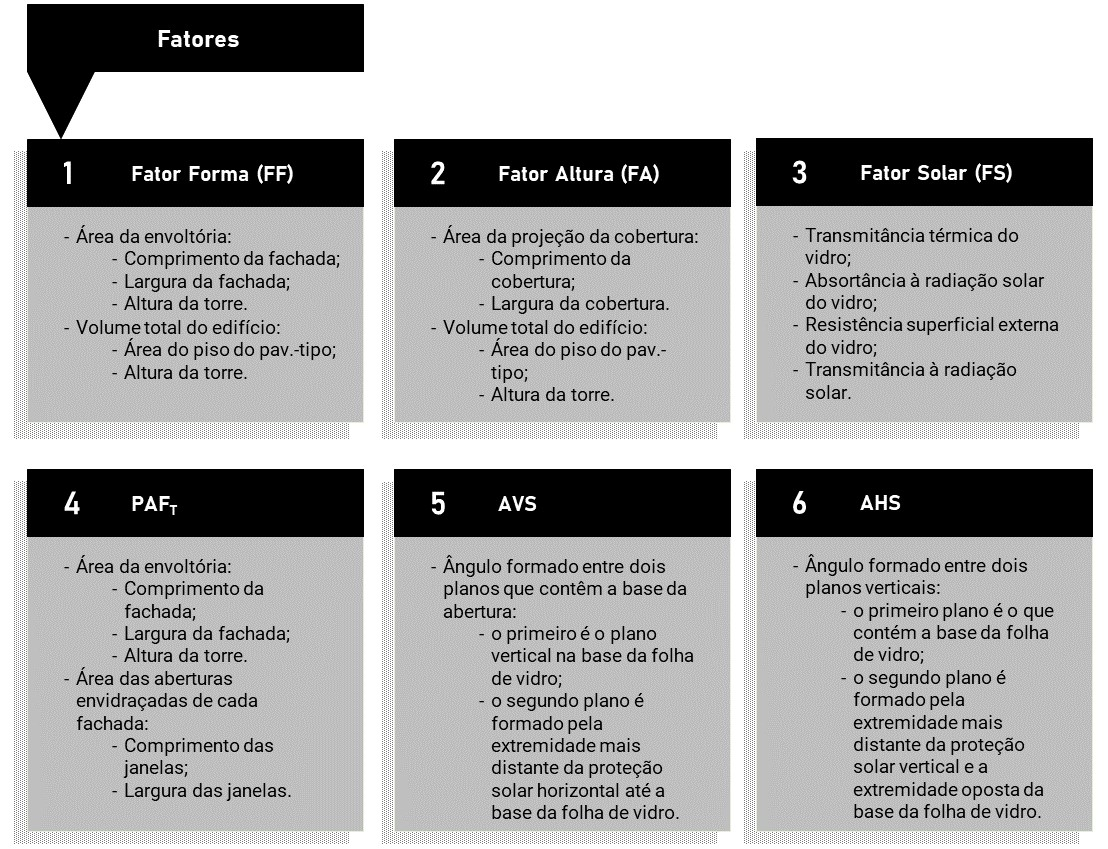
\includegraphics[width=0.8\textwidth]{figures/fig10_Fluxogramas-2.jpg}
        \begin{flushleft}
            \par \small Fonte: autor (2019)
        \end{flushleft}
        \label{fig:figura8}
    \end{figure}\vspace*{-0.6cm}

\noindent Apresentados na Tabela 7 e exemplificado na Figura \ref{fig:figura9}, os atributos estudados foram Fator de Forma, FF, Fator Altura, FA, Percentual de Área de Abertura da Fachada Total, PAFT, Ângulo Vertical de Sombreamento, AVS, e Ângulo Horizontal de Sombreamento, AHS.\vspace*{0.3cm}
\begin{figure}[H]
    \centering
    \caption{\small Estrutura arquitetônica dos modelos genéricos.}
    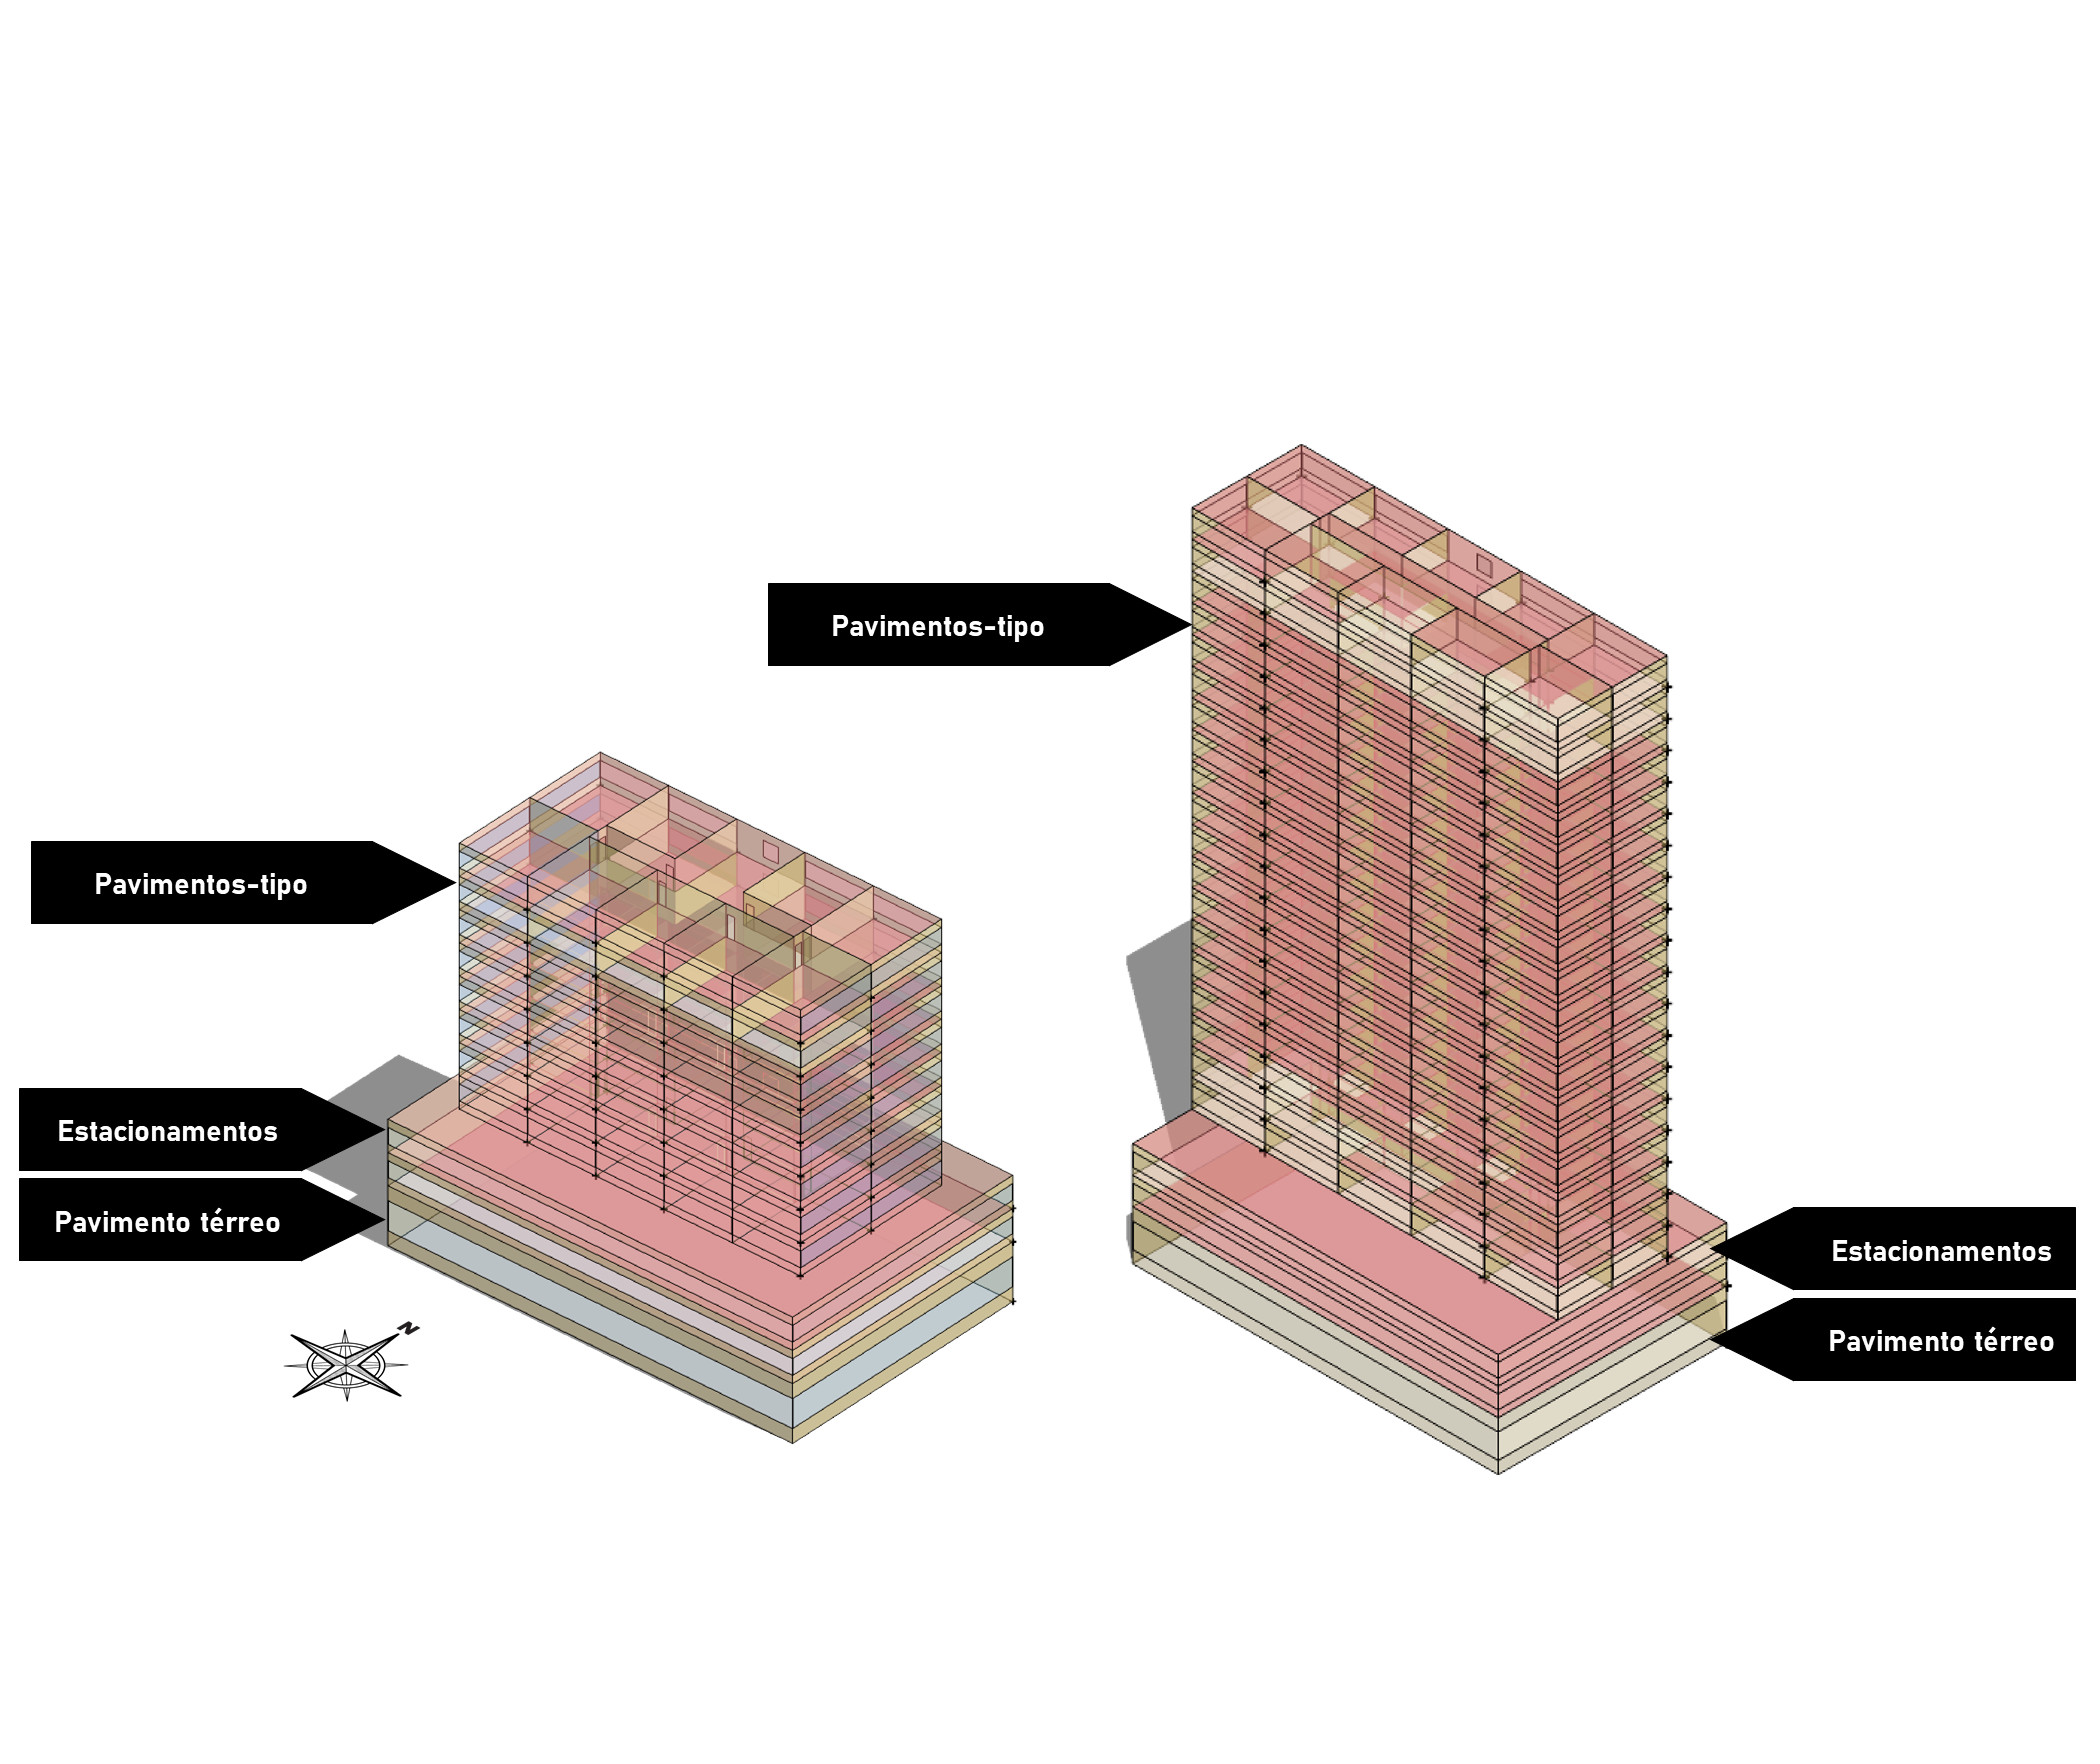
\includegraphics[width=0.9\textwidth]{figures/fig11_8-19-2pav.png}
    \begin{flushleft}
        \par \small Fonte: autor (2019).
    \end{flushleft}
    \label{fig:figura9}
\end{figure}

\noindent O PAF\textsubscript{T} e as propriedades do vidro utilizados para os modelos genéricos, como Fator Solar – FS, ou Solar Heat Gain Coefficient – SHGC, foram adotados considerando as médias desses atributos coletados in loco e complementados por dados extraídos do Catálogo de Propriedades Térmicas e Óticas de Vidro \cite{CentroBrasileirodeEficienciaEnergeticaemEdificacoesCB3E2015,AssociacaoBrasileiradeNormasTecnicas-ABNT2003}, da NBR 15220 (2003) e do INI-C \cite{InstitutoNacionaldeMetrologiaNormalizacaoeQualidadeIndustrial-INMETRO2018}, 
como forma de tornar genéricos os dados empregados, como apresentado na Tabela \ref{tab:tabela8}.%\vspace*{0.3cm} \newline
\begin{table}[H]\centering
    \caption{\small Parâmetros arquitetônicos dos modelos genéricos.}
    \vspace*{0.3cm}
    \label{tab:tabela8}
    \begin{tabular*}{\columnwidth}{@{\extracolsep{\fill}}l|ll}
    \hline
    \textbf{Parâmetro}                                                              & \textbf{Descrição}         & \textbf{Referências}  \\ \hline
    \multicolumn{3}{c}{\textbf{Dados dimensionais dos pavimentos-tipo}}\\\hline
    Número de pavimento (un)                                                        & 8                          & 19                    \\ \hline
    \makecell[l]{Proporção geométrica – pav.\\ tipo (m – Comprimento x Largura)}    & 33,75x16                   & 40x12                 \\ \hline
    Altura do pavimento-tipo (m)                                                    & 3                          & 3                     \\ \hline
    \makecell[l]{Área total construída – pavimentos-tipo (m²)}                      & 4.320                      & 9.120                 \\ \hline
    Área de projeção da cobertura - Apcob (m²)                                      & 843,75                     & 640,00                \\ \hline
    Área de projeção do edifício - Ape (m²)*                                        & 1000                       & 1000                  \\ \hline
    Área total construída - Atot (m²)                                               & 7.320                      & 12.120                \\ \hline
    Volume Total da Edificação - Vtot (m³)                                          & 24.360                     & 38.760                \\ \hline
    Área da envoltória - Aenv (m²)                                                  & 5.430,30                   & 8.890,00              \\ \hline
    Fator de Forma (FF)                                                             & 0,222                      & 0,229                 \\ \hline
    Fator Altura (FA)                                                               & 0,125                      & 0,052                 \\ \hline
    Fator Solar (FS)                                                                & 0,44                       & 0,44                  \\ \hline
    Transmitância do vidro (W/m²K)                                                  & 5,6                        & 5,6                   \\ \hline
    Área de aberturas das fachadas – Aabert (m²)                                    & 1.501,80                   & 3.152,40              \\ \hline
    PAF\textsubscript{T} (\%)                                                       & 50\%                       & 50\%                  \\ \hline
    \makecell[l]{Ângulo Vertical (AVS) e Horizontal\\ (AHS) de Sombreamento (°)}    & 0                          & 0                     \\ \hline
    \end{tabular*}
    \begin{flushleft}
        \par \small Fonte: autor (2019); *A Ape contempla a área de projeção do pavimento térreo e estacionamentos.
    \end{flushleft}
\end{table}

\noindent Segundo o INI-C, publicado pelo \textcite{InstitutoNacionaldeMetrologiaNormalizacaoeQualidadeIndustrial-INMETRO2018},
a utilização do Ângulo de Obstrução Vertical – AOV, para a simulação de obstruções solares parciais e totais são critérios opcionais que dependem da condição real levantada. Apesar da obstrução solar lateral ter sido uma condição observada em algumas edificações de Vitória, com base na observação da frequência de ocorrência, este atributo não foi considerado para o presente trabalho dada a configuração e disposição das edificações do recorte territorial em relação ao lote, que possibilitaram utilizar cenários sem obstrução solar. Além disso, para o estudo da incidência de radiação solar sobre a edificação e como ponto de partida para a implementação das estratégias passivas aos modelos genéricos, foi definido a fachada principal com orientação Sul, de acordo com a frequência de ocorrência observada na amostragem.\vspace*{0.3cm} \newline
O pavimento térreo e dois pavimentos de estacionamentos (Figura \ref{fig:figura10}), foram centralizados na base das torres em ambos os modelos, com dimensões idênticas e de forma genérica, com o intuito de evidenciar a influência sobre o consumo energético total por meio do número de pavimentos. Contudo, o uso e ocupação destas áreas se torna de baixa relevância, uma vez que as atividades de maior permanência se dão nos ambientes da torre.\vspace*{0.3cm} \newline
Estes pavimentos compreendem características arquitetônicas apresentadas em todas as edificações selecionadas em levantamento. Posteriormente, na etapa de produção de energia, foi proposto o deslocamento dos pavimentos abaixo da torre para aproveitamento de área para inserção de painéis fotovoltaicos.
\begin{figure}[H]
    \centering
    \caption{\small Conformação do pavimento térreo e estacionamentos.}
    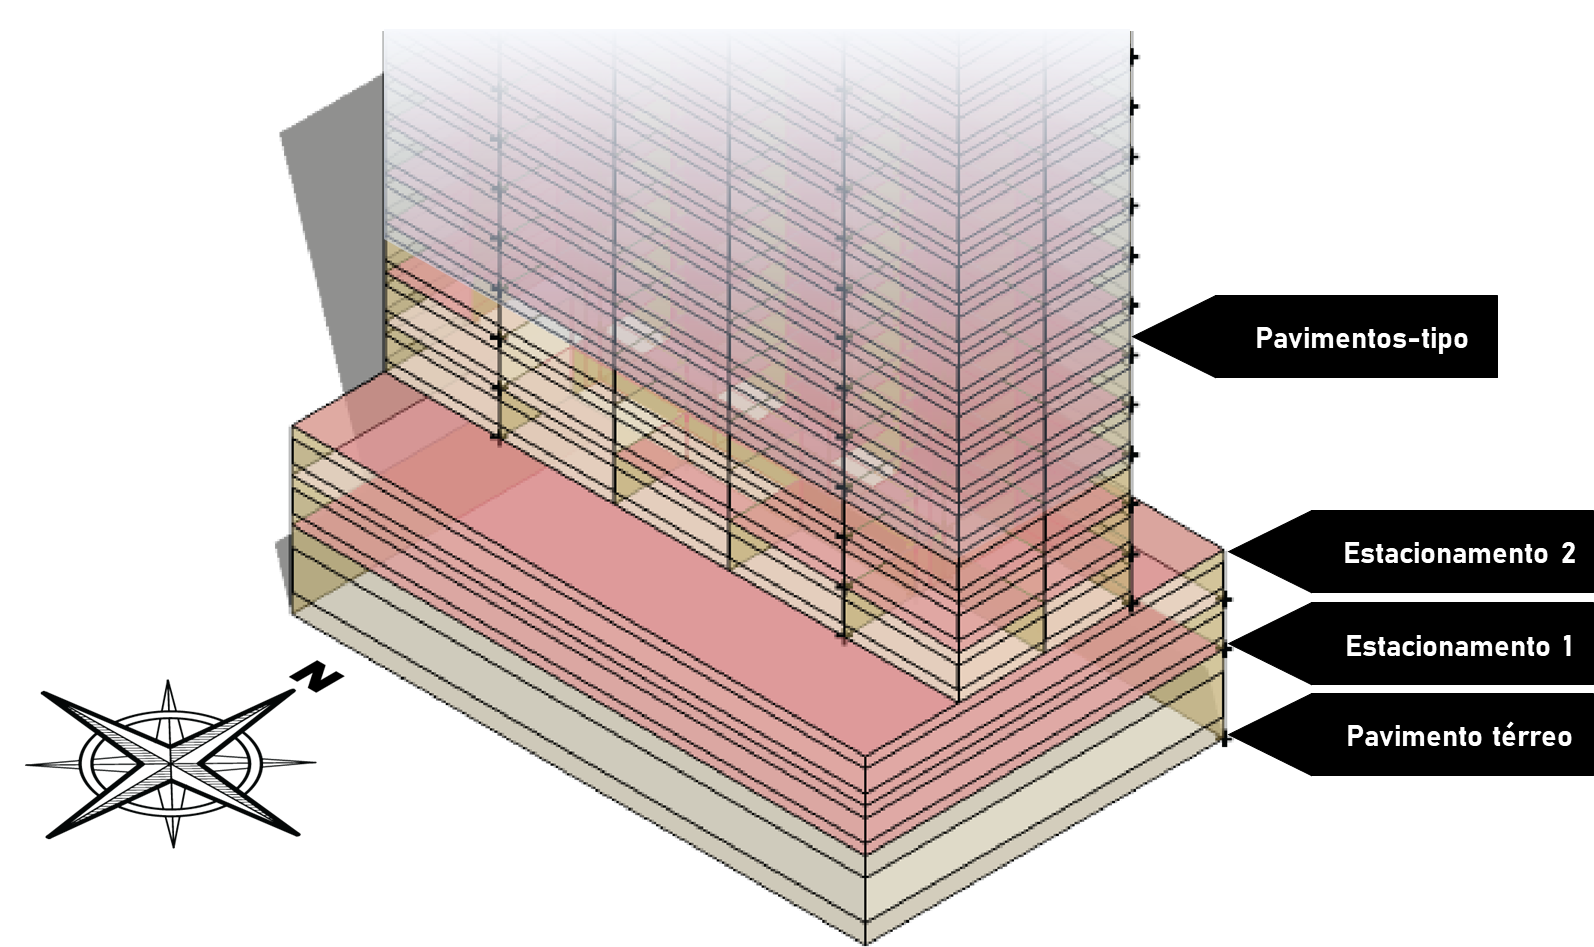
\includegraphics[width=0.9\textwidth]{figures/fig12-base_torre-1.png}
    \begin{flushleft}
        \par \small Fonte: autor (2019).
    \end{flushleft}
    \label{fig:figura10}
\end{figure}\vspace*{-0.5cm}
\noindent Os modelos são distinguidos principalmente pela área de projeção, número de pavimentos, pelo volume total e área da envoltória. Esses fatores resultam diretamente em Fator de Forma e Fator Altura distintos para cada modelo, amparando um dos objetivos específicos desta pesquisa sobre identificar as características mais influentes no consumo de energia elétrica. As zonas térmicas também formam características distintas entre os modelos genéricos, variando as áreas úteis, como apresentado na Tabela \ref{tab:tabela9}.
\begin{table}[H]
    \centering
    \caption{\small Zonas térmicas dos modelos genéricos.}
    \begin{tabular*}{\columnwidth}{@{\extracolsep{\fill}}ll}\hline
        \makecell[c]{Zonas térmicas - modelo\\ genérico de 8 pavimentos}                    & \makecell[c]{Zonas térmicas - modelo \\genérico de 19 pavimentos}                 \\ \hline
        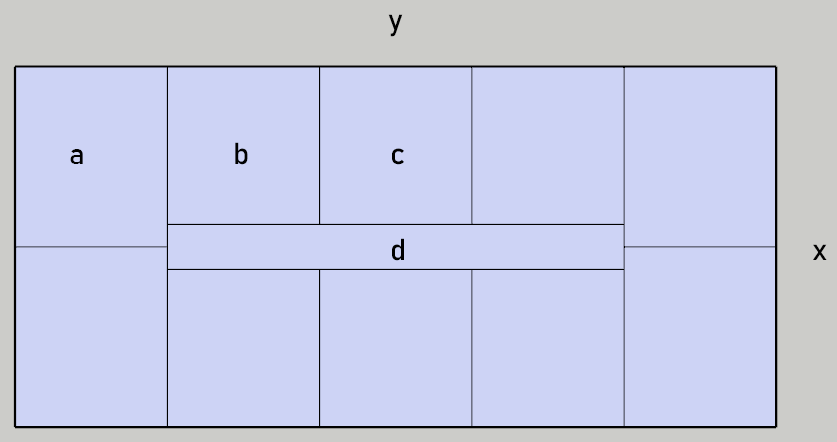
\includegraphics[width=0.5\textwidth]{figures/tab9-pb-8pav.png}                     & 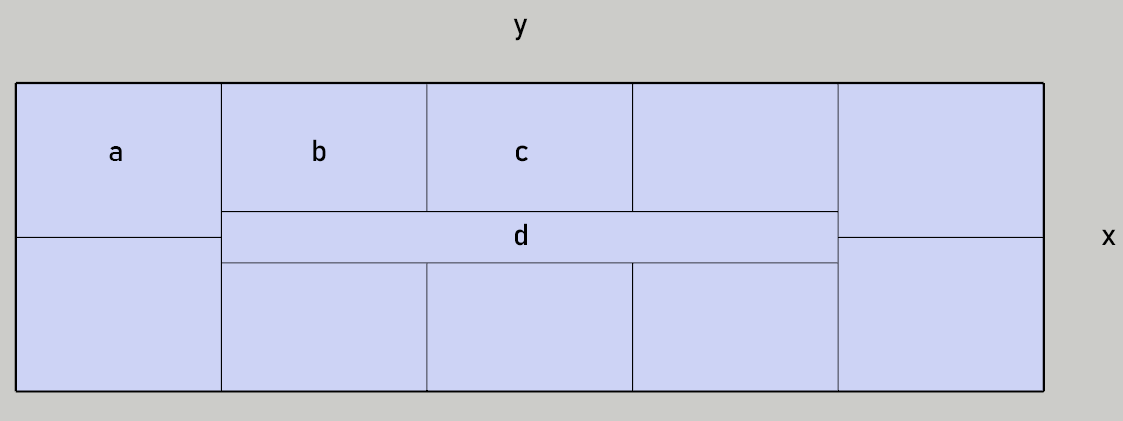
\includegraphics[width=0.5\textwidth]{figures/tab9-pb-19pav.png}                  \\
        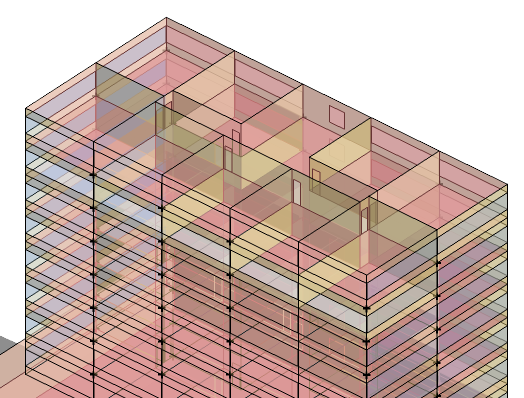
\includegraphics[width=0.5\textwidth]{figures/tab9-CEP_8pav-v3-7.png}               & 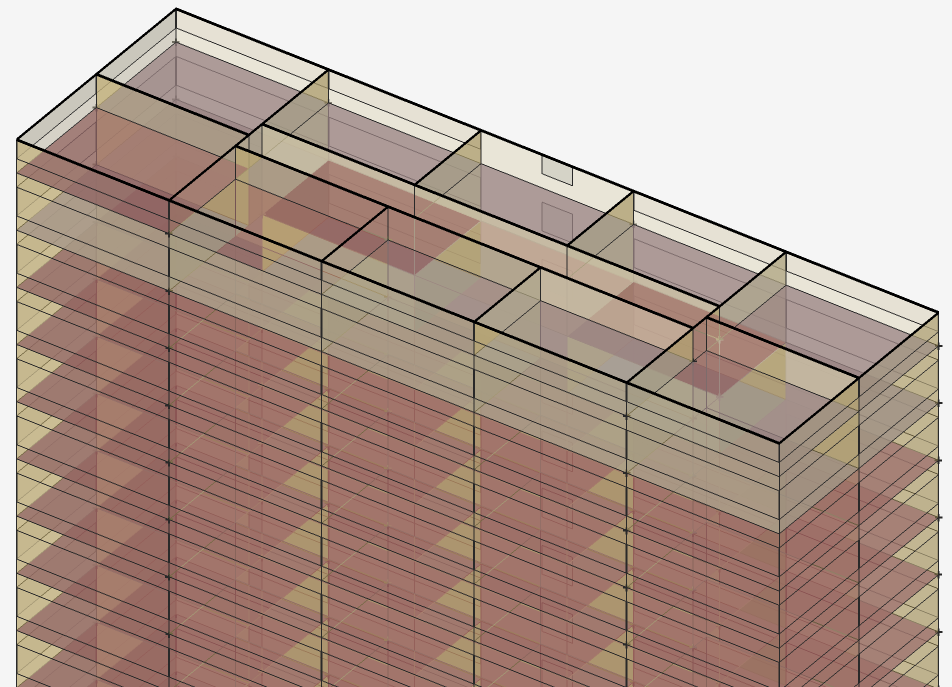
\includegraphics[width=0.5\textwidth]{figures/tab9-corte-19pav-v1.png}            \\ \hline
        Quantidade de zonas: 11                                                             & Quantidade de zonas: 11                                                           \\ \hline
        Área de projeção da torre: 843,75 m²                                                & Área de projeção da torre: 640,00 m²                                              \\ \hline
        Área da zona térmica “a”: 54,00 m²                                                  & Área da zona térmica “a”: 48,00 m²                                                \\ \hline
        Área da zona térmica “b”: 47,25 m²                                                  & Área da zona térmica “b”: 40,00 m²                                                \\ \hline
        Área da zona térmica “c+d”: 87,75 m²                                                & Área da zona térmica “c+d”: 88,00 m²                                              \\ \hline
        \makecell[l]{Largura do pavimento-tipo\\ (x): 16,00 m}                              & Largura do pavimento-tipo (x): 12,00 m                                            \\ \hline
        \makecell[l]{Comprimento do pavimento-\\tipo (y): 33,75 m}                          & \makecell[l]{Comprimento do pavimento-\\tipo (y): 40,00 m}                        \\ \hline
        \makecell[l]{Dimensões das aberturas\\ das zonas térmicas – N/S:\\ 6,70x1,51 m}     & \makecell[l]{Dimensões das aberturas das zonas\\ térmicas – N/S: 7,95x1,51 m}     \\ \hline
        \makecell[l]{Dimensões das aberturas\\ das zonas térmicas – L/O:\\ 7,95x1,51 m}     & \makecell[l]{Dimensões das aberturas das zonas\\ térmicas – L/O: 5,95x1,51 m}     \\ \hline
        \makecell[l]{Dimensões das aberturas\\ das zonas térmicas – circ.:\\ 1,49x1,51 m}   & \makecell[l]{Dimensões das aberturas das zonas\\ térmicas – circ.: 1,49x1,51 m}   \\ \hline
        \multicolumn{2}{l}{Dimensões das zonas térmicas – Pav. térreo e garagens: 40 x 25 m}                                                                                    \\ \hline
        \multicolumn{2}{l}{\makecell[l]{Dimensões das aberturas das zonas térmicas – Pav.\\ térreo e gar.: 39,95x1,51 m (N/S); 24,95x1,51 m (L/O)}}                             \\ \hline
    \end{tabular*}
    \begin{flushleft}
        \par \small Fonte: autor (2019).
    \end{flushleft}
    \label{tab:tabela9}
\end{table}

\noindent Foram propostas, na etapa de otimização, proteções solares horizontais para as aberturas, que servem como proteção à radiação solar direta e controle de iluminação natural em horários predeterminados – 9, 12 e 15 horas. Este controle de horários de incidência solar se deu pelo comprimento das proteções solares propostas. Esta solução foi adotada como estratégia passiva. Utilizou-se, também, a área para proteção solar como espaço para exploração de energia solar por meio de painéis fotovoltaicos sobre os elementos protetores, como exemplificado na Figura \ref{fig:figura11} \cite{Didone2014a}.
\begin{figure}[H]
    \centering
    \caption{\small Painéis fotovoltaicos sobre as proteções solares da fachada oeste e cobertura.}
    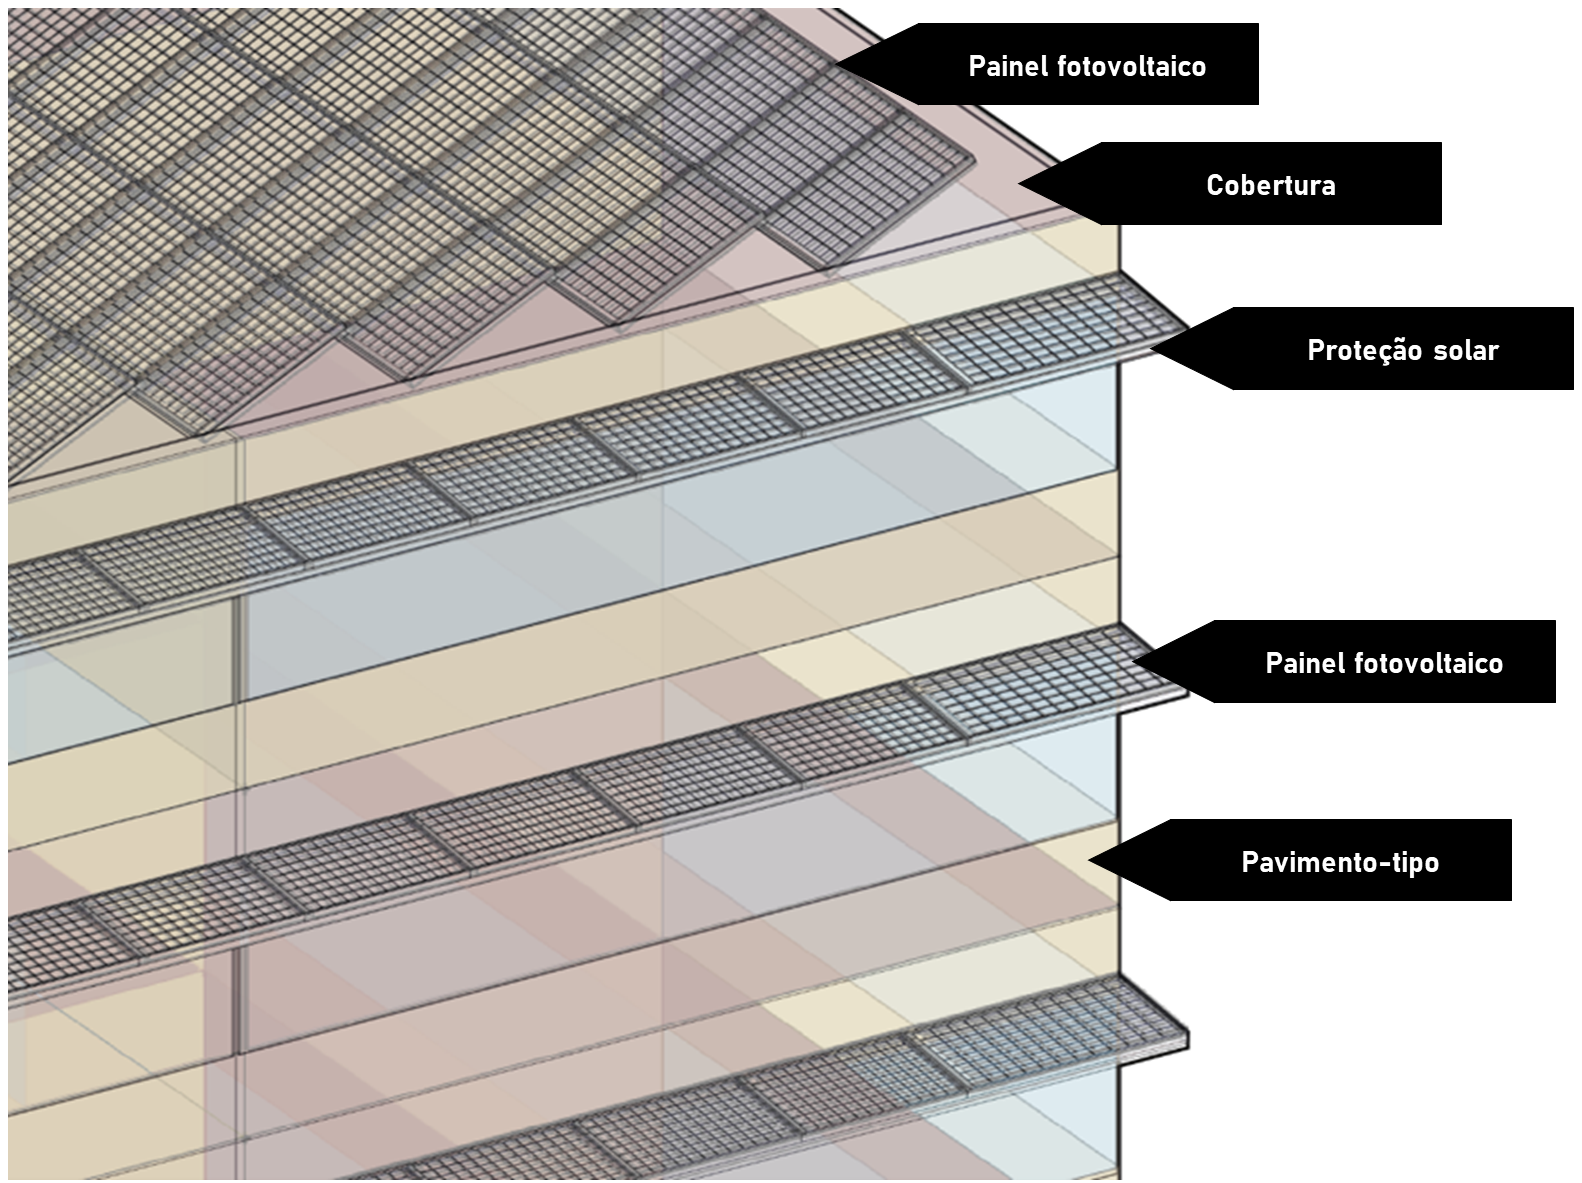
\includegraphics[width=0.9\textwidth]{figures/fig13-paineis pv.png}
    \begin{flushleft}
        \par \small Fonte: autor (2019).
    \end{flushleft}
    \label{fig:figura11}
\end{figure}

\subsubsection{Parâmetros arquitetônicos dos modelos genéricos}
\noindent A preparação para o início das simulações é precedida pela definição dos parâmetros arquitetônicos e das variáveis contidas em cada um destes. Com base no levantamento in loco e no referencial teórico, são inicialmente modificados os atributos arquitetônicos em três fases: envoltória, sistemas de iluminação e condicionamento de ar. As modificações foram implementadas de forma ordenada, a fim de evidenciar a influência de cada medida proposta no consumo final de energia elétrica da edificação genérica. As medidas propostas para analise por meio de simulação computacional estão apresentadas na Tabela \ref{tab:tabela10}.
\begin{table}[H]
    \centering
    \footnotesize
    \caption{\small Zonas térmicas dos modelos genéricos.}\vspace*{0.3cm}
    \begin{tabular*}{\columnwidth}{@{\extracolsep{\fill}}clcrl}\hline
        \multicolumn{2}{c}{\textbf{Parâmetros}}                                                                                              & \multicolumn{2}{c}{\textbf{Variáveis}}   & \textbf{Descrição}\\\hline
        \multirow{4}{*}{1}  & \multirow{4}{*}{Orientação Solar}                                                                              & a                  & 0°                  & \multirow{4}{*}{Orientação solar final da fachada principal.}\\
                            &                                                                                                                & b                  & 90°                 & \\
                            &                                                                                                                & c                  & 180°                & \\
                            &                                                                                                                & d                  & 360°                & \\\hline
        \multirow{4}{*}{2}  & \multirow{4}{*}{Vidro com baixo Fator Solar}                                                                   &                    &                     & \multirow{4}{*}{\makecell[l]{Foram simuladas duas situações aplicas aos\\
                                                                                                                                                                                         modelos genéricos: a primeira utilizando\\ o vidro
                                                                                                                                                                                         levantado in loco (a) e o modelo mais\\ eficiente
                                                                                                                                                                                         comercializado\\ no mercado brasileiro (b) (CB3E; ABIVIDRO, 2015).}}\\
                            &                                                                                                                & a                  & FS: 0,44            & \\
                            &                                                                                                                &                    &                     & \\
                            &                                                                                                                & b                  & FS: 0,16            & \\\hline
        \multirow{3}{*}{3}  & \multirow{3}{*}{\makecell[l]{Percentual de Área de Abertura\\ da Fachada Total – PAF\textsubscript{T}}}        & a                  & 30\%                & \multirow{3}{*}{\makecell[l]{As aberturas das fachadas foram definidas de\\
                                                                                                                                                                                            acordo com as indicações de programas de                                                                                                                                                                                             economia de energia como PROCEL EDIFICA e o\\
                                                                                                                                                                                            Advanced Energy Design Guide for Small to\\
                                                                                                                                                                                            Medium Office Buildings (Guia Avançado de\\
                                                                                                                                                                                            Planejamento Energético para Edificações de\\
                                                                                                                                                                                            Escritório de Pequeno e Médio Porte) da ASHRAE\\
                                                                                                                                                                                            (ASHRAE et al., 2014, 2019; FERRADOR FILHO;\\
                                                                                                                                                                                            AGUIAR; KNIESS, 2018).}}\\
                            &                                                                                                                & b                  & 50\%                & \\
                            &                                                                                                                & c                  & 80\%                & \\\hline
    \end{tabular*}
    \begin{flushleft}
        \par \small Fonte: autor (2019).
    \end{flushleft}
    \label{tab:tabela10}
\end{table}


\end{onehalfspace}